% Created by tikzDevice version 0.10.1 on 2016-04-22 17:26:10
% !TEX encoding = UTF-8 Unicode
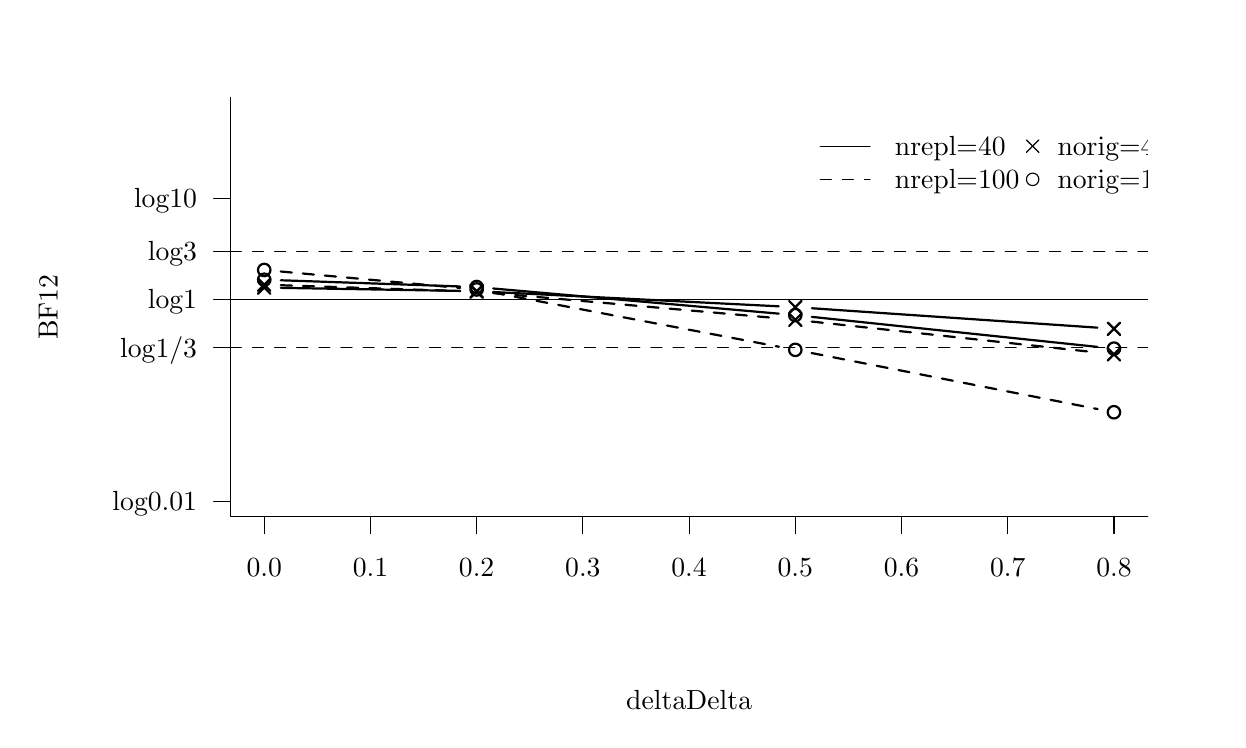
\begin{tikzpicture}[x=1pt,y=1pt]
\definecolor{fillColor}{RGB}{255,255,255}
\path[use as bounding box,fill=fillColor,fill opacity=0.00] (0,0) rectangle (430.00,250.00);
\begin{scope}
\path[clip] ( 73.20, 73.20) rectangle (404.80,224.80);
\definecolor{drawColor}{RGB}{0,0,0}

\path[draw=drawColor,line width= 0.8pt,line join=round,line cap=round] ( 91.48,155.98) -- (156.24,154.88);

\path[draw=drawColor,line width= 0.8pt,line join=round,line cap=round] (168.23,154.48) -- (271.39,149.31);

\path[draw=drawColor,line width= 0.8pt,line join=round,line cap=round] (283.37,148.61) -- (386.53,141.60);

\path[draw=drawColor,line width= 0.8pt,line join=round,line cap=round] ( 83.23,153.84) -- ( 87.73,158.34);

\path[draw=drawColor,line width= 0.8pt,line join=round,line cap=round] ( 83.23,158.34) -- ( 87.73,153.84);

\path[draw=drawColor,line width= 0.8pt,line join=round,line cap=round] (159.99,152.53) -- (164.49,157.03);

\path[draw=drawColor,line width= 0.8pt,line join=round,line cap=round] (159.99,157.03) -- (164.49,152.53);

\path[draw=drawColor,line width= 0.8pt,line join=round,line cap=round] (275.13,146.76) -- (279.63,151.26);

\path[draw=drawColor,line width= 0.8pt,line join=round,line cap=round] (275.13,151.26) -- (279.63,146.76);

\path[draw=drawColor,line width= 0.8pt,line join=round,line cap=round] (390.27,138.95) -- (394.77,143.45);

\path[draw=drawColor,line width= 0.8pt,line join=round,line cap=round] (390.27,143.45) -- (394.77,138.95);
\end{scope}
\begin{scope}
\path[clip] (  0.00,  0.00) rectangle (430.00,250.00);
\definecolor{drawColor}{RGB}{0,0,0}

\path[draw=drawColor,line width= 0.4pt,line join=round,line cap=round] ( 73.20,224.80) --
	( 73.20, 73.20) --
	(404.80, 73.20);
\end{scope}
\begin{scope}
\path[clip] (  0.00,  0.00) rectangle (430.00,250.00);
\definecolor{drawColor}{RGB}{0,0,0}

\node[text=drawColor,anchor=base,inner sep=0pt, outer sep=0pt, scale=  1.00] at (239.00,  3.60) {deltaDelta};

\node[text=drawColor,rotate= 90.00,anchor=base,inner sep=0pt, outer sep=0pt, scale=  1.00] at ( 10.80,149.00) {BF12};
\end{scope}
\begin{scope}
\path[clip] ( 73.20, 73.20) rectangle (404.80,224.80);
\definecolor{drawColor}{RGB}{0,0,0}

\path[draw=drawColor,line width= 0.8pt,dash pattern=on 4pt off 4pt ,line join=round,line cap=round] ( 91.48,156.93) -- (156.24,154.82);

\path[draw=drawColor,line width= 0.8pt,dash pattern=on 4pt off 4pt ,line join=round,line cap=round] (168.22,154.09) -- (271.40,144.98);

\path[draw=drawColor,line width= 0.8pt,dash pattern=on 4pt off 4pt ,line join=round,line cap=round] (283.34,143.80) -- (386.55,132.61);

\path[draw=drawColor,line width= 0.8pt,line join=round,line cap=round] ( 83.23,154.87) -- ( 87.73,159.37);

\path[draw=drawColor,line width= 0.8pt,line join=round,line cap=round] ( 83.23,159.37) -- ( 87.73,154.87);

\path[draw=drawColor,line width= 0.8pt,line join=round,line cap=round] (159.99,152.37) -- (164.49,156.87);

\path[draw=drawColor,line width= 0.8pt,line join=round,line cap=round] (159.99,156.87) -- (164.49,152.37);

\path[draw=drawColor,line width= 0.8pt,line join=round,line cap=round] (275.13,142.20) -- (279.63,146.70);

\path[draw=drawColor,line width= 0.8pt,line join=round,line cap=round] (275.13,146.70) -- (279.63,142.20);

\path[draw=drawColor,line width= 0.8pt,line join=round,line cap=round] (390.27,129.72) -- (394.77,134.22);

\path[draw=drawColor,line width= 0.8pt,line join=round,line cap=round] (390.27,134.22) -- (394.77,129.72);

\path[draw=drawColor,line width= 0.8pt,line join=round,line cap=round] ( 91.48,158.72) -- (156.24,156.49);

\path[draw=drawColor,line width= 0.8pt,line join=round,line cap=round] (168.22,155.75) -- (271.40,146.66);

\path[draw=drawColor,line width= 0.8pt,line join=round,line cap=round] (283.35,145.50) -- (386.55,134.65);

\path[draw=drawColor,line width= 0.8pt,line join=round,line cap=round] ( 85.48,158.92) circle (  2.25);

\path[draw=drawColor,line width= 0.8pt,line join=round,line cap=round] (162.24,156.28) circle (  2.25);

\path[draw=drawColor,line width= 0.8pt,line join=round,line cap=round] (277.38,146.13) circle (  2.25);

\path[draw=drawColor,line width= 0.8pt,line join=round,line cap=round] (392.52,134.02) circle (  2.25);

\path[draw=drawColor,line width= 0.8pt,dash pattern=on 4pt off 4pt ,line join=round,line cap=round] ( 91.46,161.89) -- (156.27,155.94);

\path[draw=drawColor,line width= 0.8pt,dash pattern=on 4pt off 4pt ,line join=round,line cap=round] (168.14,154.28) -- (271.48,134.70);

\path[draw=drawColor,line width= 0.8pt,dash pattern=on 4pt off 4pt ,line join=round,line cap=round] (283.27,132.43) -- (386.63,112.18);

\path[draw=drawColor,line width= 0.8pt,line join=round,line cap=round] ( 85.48,162.44) circle (  2.25);

\path[draw=drawColor,line width= 0.8pt,line join=round,line cap=round] (162.24,155.40) circle (  2.25);

\path[draw=drawColor,line width= 0.8pt,line join=round,line cap=round] (277.38,133.58) circle (  2.25);

\path[draw=drawColor,line width= 0.8pt,line join=round,line cap=round] (392.52,111.03) circle (  2.25);

\path[] (277.38,219.19) rectangle (362.90,183.19);

\path[draw=drawColor,line width= 0.4pt,line join=round,line cap=round] (286.38,207.19) -- (304.38,207.19);

\path[draw=drawColor,line width= 0.4pt,dash pattern=on 4pt off 4pt ,line join=round,line cap=round] (286.38,195.19) -- (304.38,195.19);

\node[text=drawColor,anchor=base west,inner sep=0pt, outer sep=0pt, scale=  1.00] at (313.38,203.74) {nrepl=40};

\node[text=drawColor,anchor=base west,inner sep=0pt, outer sep=0pt, scale=  1.00] at (313.38,191.74) {nrepl=100};

\path[] (354.14,219.19) rectangle (421.66,183.19);

\path[draw=drawColor,line width= 0.4pt,line join=round,line cap=round] (360.89,204.94) -- (365.39,209.44);

\path[draw=drawColor,line width= 0.4pt,line join=round,line cap=round] (360.89,209.44) -- (365.39,204.94);

\path[draw=drawColor,line width= 0.4pt,line join=round,line cap=round] (363.14,195.19) circle (  2.25);

\node[text=drawColor,anchor=base west,inner sep=0pt, outer sep=0pt, scale=  1.00] at (372.14,203.74) {norig=40};

\node[text=drawColor,anchor=base west,inner sep=0pt, outer sep=0pt, scale=  1.00] at (372.14,191.74) {norig=100};
\end{scope}
\begin{scope}
\path[clip] (  0.00,  0.00) rectangle (430.00,250.00);
\definecolor{drawColor}{RGB}{0,0,0}

\path[draw=drawColor,line width= 0.4pt,line join=round,line cap=round] ( 85.48, 73.20) -- (392.52, 73.20);

\path[draw=drawColor,line width= 0.4pt,line join=round,line cap=round] ( 85.48, 73.20) -- ( 85.48, 67.20);

\path[draw=drawColor,line width= 0.4pt,line join=round,line cap=round] (123.86, 73.20) -- (123.86, 67.20);

\path[draw=drawColor,line width= 0.4pt,line join=round,line cap=round] (162.24, 73.20) -- (162.24, 67.20);

\path[draw=drawColor,line width= 0.4pt,line join=round,line cap=round] (200.62, 73.20) -- (200.62, 67.20);

\path[draw=drawColor,line width= 0.4pt,line join=round,line cap=round] (239.00, 73.20) -- (239.00, 67.20);

\path[draw=drawColor,line width= 0.4pt,line join=round,line cap=round] (277.38, 73.20) -- (277.38, 67.20);

\path[draw=drawColor,line width= 0.4pt,line join=round,line cap=round] (315.76, 73.20) -- (315.76, 67.20);

\path[draw=drawColor,line width= 0.4pt,line join=round,line cap=round] (354.14, 73.20) -- (354.14, 67.20);

\path[draw=drawColor,line width= 0.4pt,line join=round,line cap=round] (392.52, 73.20) -- (392.52, 67.20);

\node[text=drawColor,anchor=base,inner sep=0pt, outer sep=0pt, scale=  1.00] at ( 85.48, 51.60) {0.0};

\node[text=drawColor,anchor=base,inner sep=0pt, outer sep=0pt, scale=  1.00] at (123.86, 51.60) {0.1};

\node[text=drawColor,anchor=base,inner sep=0pt, outer sep=0pt, scale=  1.00] at (162.24, 51.60) {0.2};

\node[text=drawColor,anchor=base,inner sep=0pt, outer sep=0pt, scale=  1.00] at (200.62, 51.60) {0.3};

\node[text=drawColor,anchor=base,inner sep=0pt, outer sep=0pt, scale=  1.00] at (239.00, 51.60) {0.4};

\node[text=drawColor,anchor=base,inner sep=0pt, outer sep=0pt, scale=  1.00] at (277.38, 51.60) {0.5};

\node[text=drawColor,anchor=base,inner sep=0pt, outer sep=0pt, scale=  1.00] at (315.76, 51.60) {0.6};

\node[text=drawColor,anchor=base,inner sep=0pt, outer sep=0pt, scale=  1.00] at (354.14, 51.60) {0.7};

\node[text=drawColor,anchor=base,inner sep=0pt, outer sep=0pt, scale=  1.00] at (392.52, 51.60) {0.8};

\path[draw=drawColor,line width= 0.4pt,line join=round,line cap=round] ( 73.20, 78.81) -- ( 73.20,188.33);

\path[draw=drawColor,line width= 0.4pt,line join=round,line cap=round] ( 73.20, 78.81) -- ( 67.20, 78.81);

\path[draw=drawColor,line width= 0.4pt,line join=round,line cap=round] ( 73.20,134.41) -- ( 67.20,134.41);

\path[draw=drawColor,line width= 0.4pt,line join=round,line cap=round] ( 73.20,151.83) -- ( 67.20,151.83);

\path[draw=drawColor,line width= 0.4pt,line join=round,line cap=round] ( 73.20,169.25) -- ( 67.20,169.25);

\path[draw=drawColor,line width= 0.4pt,line join=round,line cap=round] ( 73.20,188.33) -- ( 67.20,188.33);

\node[text=drawColor,anchor=base east,inner sep=0pt, outer sep=0pt, scale=  1.00] at ( 61.20, 75.37) {log0.01};

\node[text=drawColor,anchor=base east,inner sep=0pt, outer sep=0pt, scale=  1.00] at ( 61.20,130.97) {log1/3};

\node[text=drawColor,anchor=base east,inner sep=0pt, outer sep=0pt, scale=  1.00] at ( 61.20,148.38) {log1};

\node[text=drawColor,anchor=base east,inner sep=0pt, outer sep=0pt, scale=  1.00] at ( 61.20,165.80) {log3};

\node[text=drawColor,anchor=base east,inner sep=0pt, outer sep=0pt, scale=  1.00] at ( 61.20,184.89) {log10};
\end{scope}
\begin{scope}
\path[clip] ( 73.20, 73.20) rectangle (404.80,224.80);
\definecolor{drawColor}{RGB}{0,0,0}

\path[draw=drawColor,line width= 0.4pt,line join=round,line cap=round] ( 73.20,151.83) -- (404.80,151.83);

\path[draw=drawColor,line width= 0.4pt,dash pattern=on 4pt off 4pt ,line join=round,line cap=round] ( 73.20,134.41) -- (404.80,134.41);

\path[draw=drawColor,line width= 0.4pt,dash pattern=on 4pt off 4pt ,line join=round,line cap=round] ( 73.20,169.25) -- (404.80,169.25);
\end{scope}
\end{tikzpicture}
